\documentclass[12pt]{article}
\usepackage{amsmath,amssymb,amsthm}
\usepackage{graphicx}

% For url formatting and hyperlinks
%\usepackage{url}
\usepackage[colorlinks=true,urlcolor=blue]{hyperref}
\urlstyle{sf}

\title{Syllabus for Computational OR}
\author{Ryo Kimura}
%\date{February 12, 2019}
\begin{document}
\maketitle

\begin{center}
    
\includegraphics[height=2in]{computer-green-unix-large.png}
    \hspace{0.5in}
    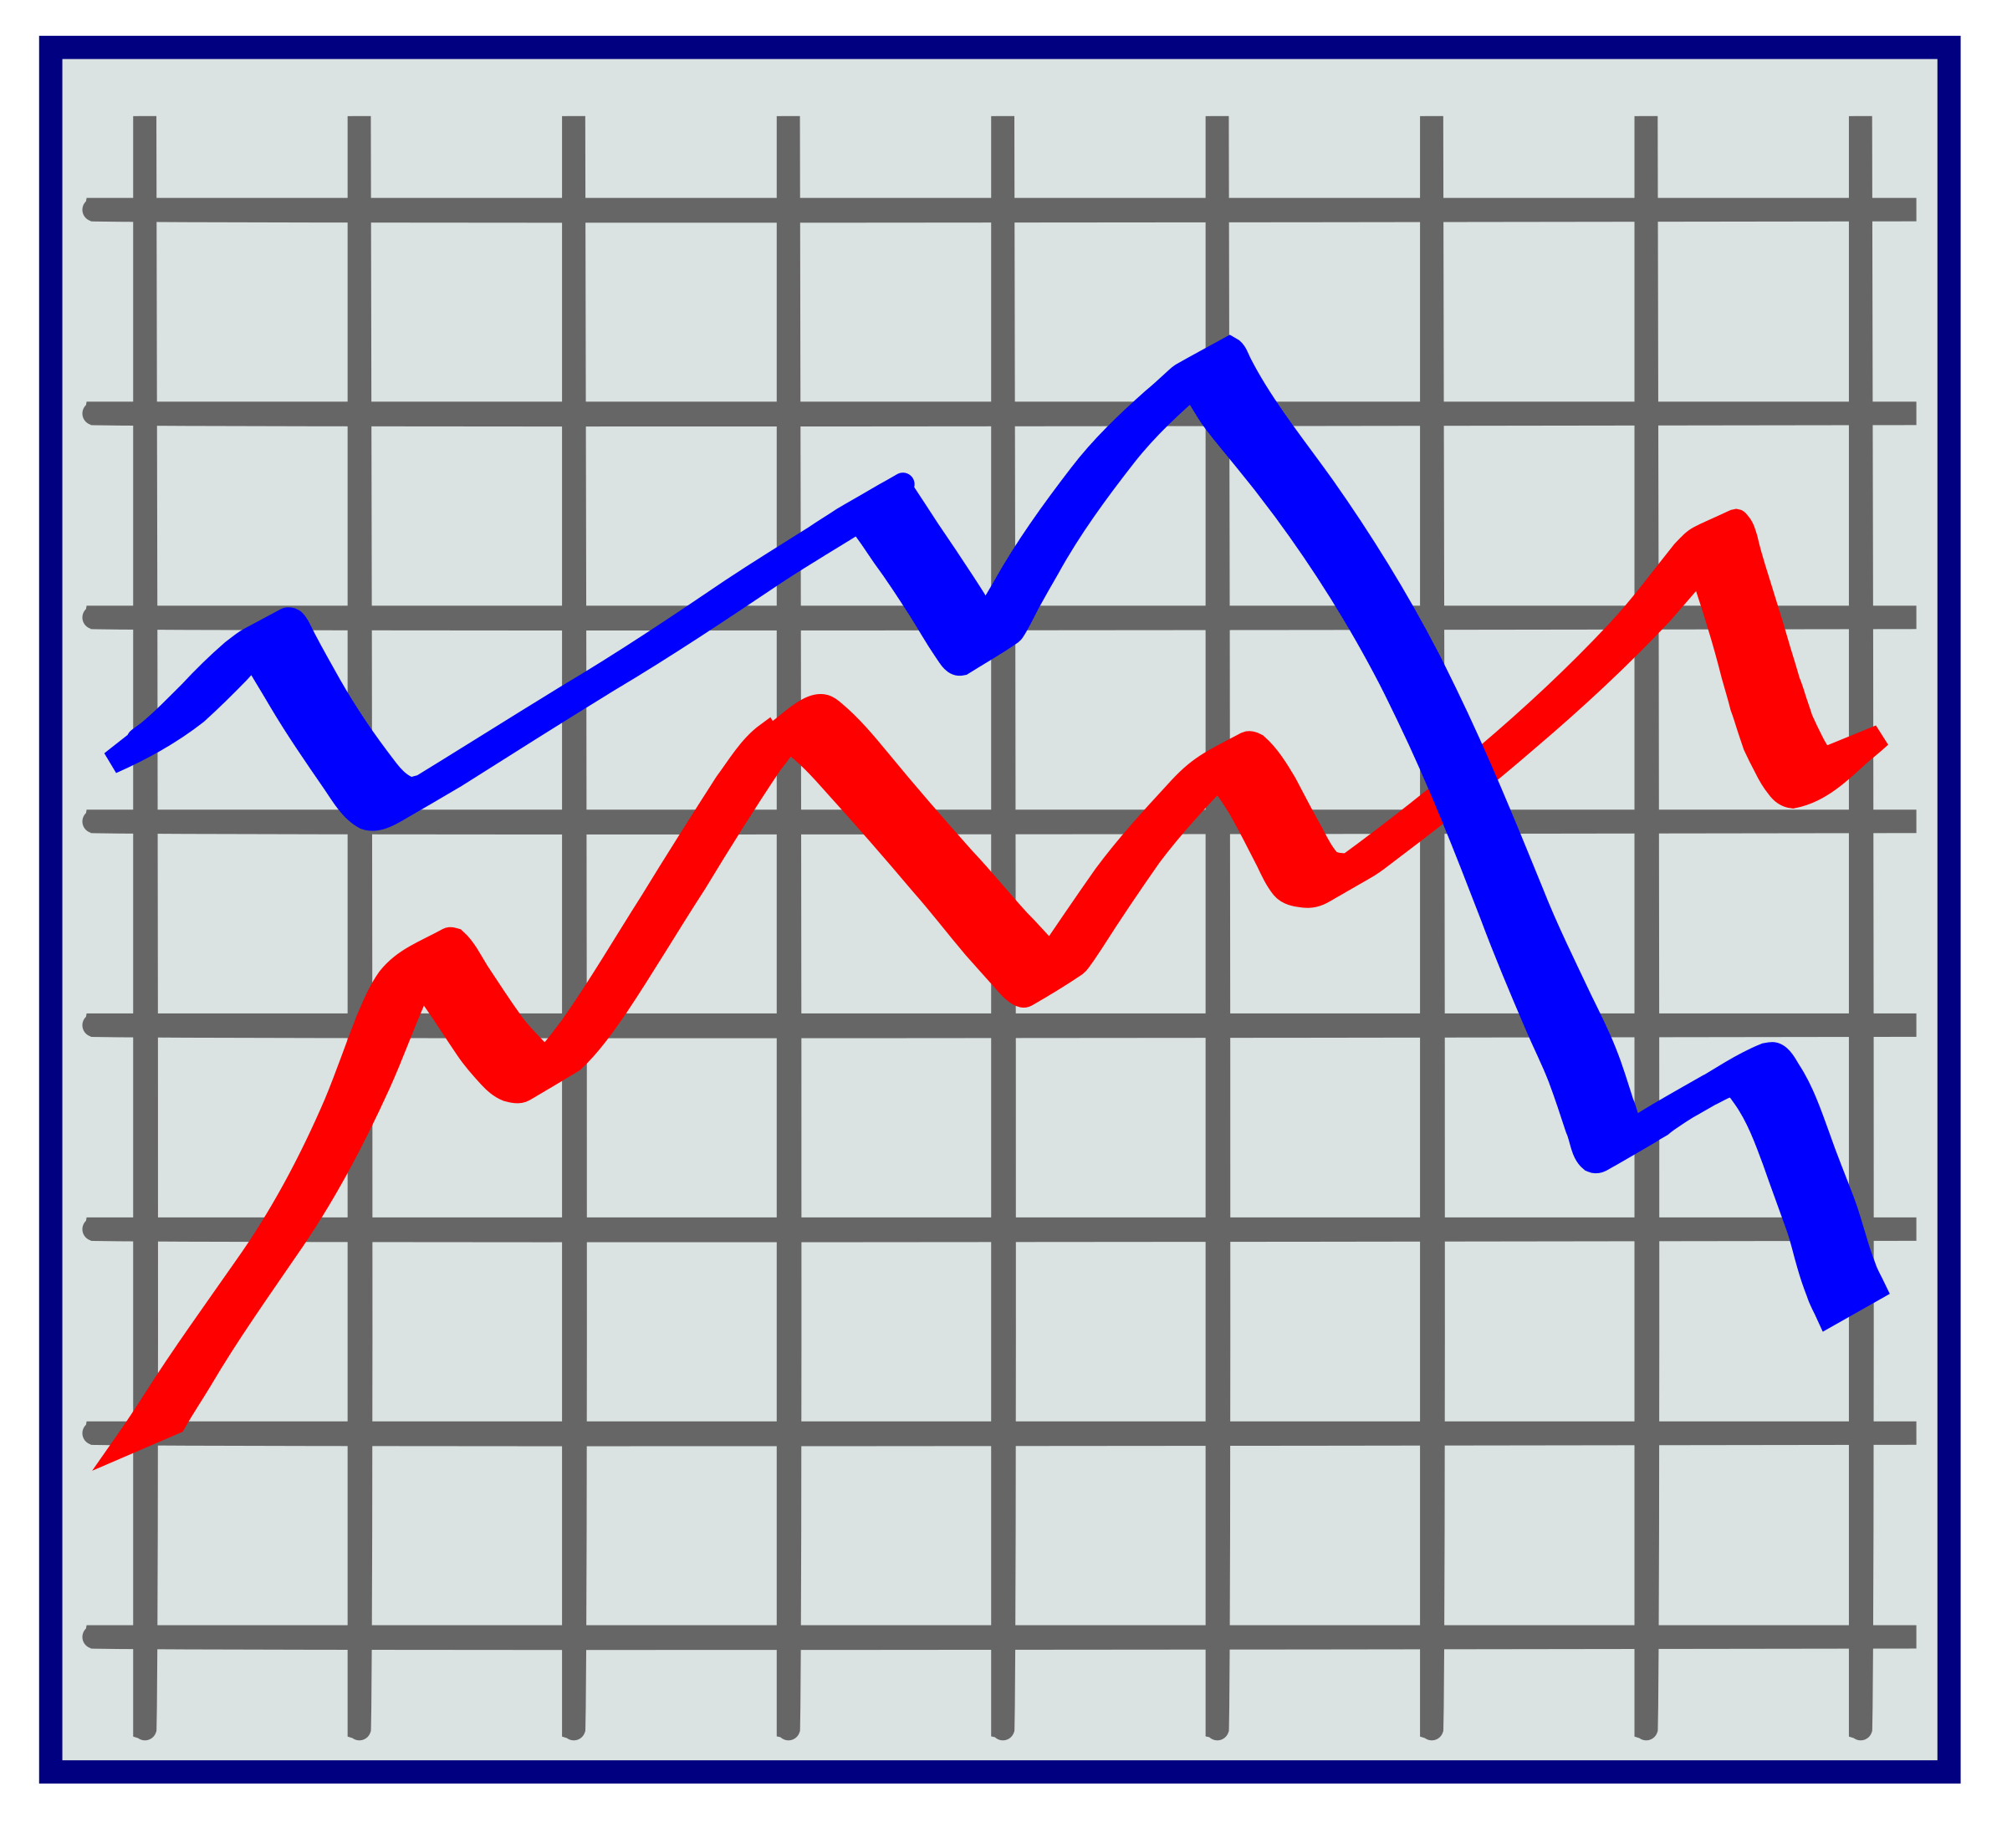
\includegraphics[height=2in]{xoseluis-xoseluis-grafica1-large.png}
\end{center}
\section*{Course Description}
Computational experiments are a vital component of many operations research (OR) projects, providing empirical justification and practical insights for theoretical results. This course covers the key practical aspects of designing and conducting computational experiments in optimization, including model implementation, design and analysis of computational experiments, and customization of solver behavior (especially in implementing decomposition methods). We use mixed integer programming (MIP) models as our main framework. While this course is not meant to provide an introduction to coding, we will also briefly cover good coding practice.

\section*{Topics}
\begin{itemize}
    \item \textbf{Coding Practice}: fundamentals, coding tools (build systems, version control, documentation), debugging (debuggers, unit testing)
    \item \textbf{Model Implementation}: optimization solvers, basic implementation, solver parameters, modular design (DMAS framework)
    \item \textbf{Computational Experiments}: test instances, running experiments (metrics, timing, logging/parsing), performance analysis/plots
    \item \textbf{Solver Customization}: implementing decomposition methods (Dantzig-Wolfe, Benders, Lagrangian decomposition), callbacks (user/lazy cuts, primal heuristics, termination), branch-cut-and-price
\end{itemize}
In addition, one or more of the following topics may also be covered: modeling languages (AMPL/GAMS/OPL, JuMP), convex optimization (Mosek/CVX), constraint programming (CPO/Gecode, constraint-based scheduling, custom constraints), machine learning (scikit-learn/TensorFlow)
%, quantum computing (D-Wave, IBM Q/Qiskit)
%, metaheuristics (tabu search, simulated/quantum annealing, large neighborhood search, late acceptance hill climbing)
\subsection*{Prerequisites}
This course assumes familiarity with basic MIP models and some coding background (at least one introductory programming course or equivalent). In addition, modules 10-12 assume slightly more background in integer programming (i.e., branch-and-bound and decomposition methods).
\section*{References}
All course materials (tutorials/articles, relevant links, example code) will be posted on the course Canvas site. In addition to the references listed in the tutorials, the following references may be useful throughout the course:
\begin{itemize}
    \item Winston, W. L., \emph{Operations Research: Applications and Algorithms}, 4th Ed. (Cengage Learning, 2004) - \textbf{OR modeling}
    \item Severance, C., \emph{Python for Everybody} (\url{https://books.trinket.io/pfe/}) - \textbf{Python programming}
    \item Conforti, M., Cornu\'{e}jols, G., and Zambelli, G., \emph{Integer Programming} (Springer, 2014) - \textbf{integer programming theory}
    %\item \emph{LearnC++} (\url{https://www.learncpp.com}) - \textbf{C++ programming}
    %\item Course page for \emph{ORIE 6125: Computational Methods in Operations Research} (Patrick Steele, Cornell) - \textbf{coding practice}
    %\item Berberich, Hagen, Hiller, and Moser, Chapter 8. Experiments, \emph{Algorithm Engineering: Bridging the Gap Between Algorithm, Theory, and Practice} - \textbf{computational experiments}
    %\item Ralphs et. al., \emph{Decomposition Methods for Discrete Optimization} - \textbf{decomposition methods}
\end{itemize}
%Kendall et al, Good Laboratory Practice for optimization research
%*Algorithm Engineering: Bridging the Gap Between Algorithm Theory and Practice

\section*{Course Format and Evaluation}
This course does not have scheduled class sessions/lectures. Instead, the instructor will upload tutorials/articles, relevant links, and example code to the course Canvas site weekly, which students will be expected to read in a timely manner.

Students are required to submit a course project utilizing computational OR. They may select a project from a number of predefined options, or they may propose their own project which can be aligned with their research.

\section*{Tentative Course Outline}
\begin{table}[h!]
\begin{tabular}{|l|l|}
    \hline
    Module 1 & Fundamentals (SSH/SFTP, Linux, Bash, Python, C++) \\
    Module 2 & Optimization Software (problem classes, Gurobi, CPLEX) \\
    Module 3 & Basic Modeling (IP review, basic implementation, output) \\
    Module 4 & Modular Modeling (DMAS framework, solver parameters) \\
    Module 5 & Coding Tools (Git, Make/CMake, Sphinx/Doxygen) \\
    Module 6 & Debugging (reading documentation, pdb/GDB, unit testing) \\
    Module 7 & Test Instances (data wrangling, random generation) \\
    Module 8 & Running Experiments (metrics, timing, logging/parsing) \\
    Module 9 & Analyzing Experiments (pandas, performance plots) \\
    Module 10 & Using Decompositions (Dantzig-Wolfe, Benders, Lagrangian) \\
    Module 11 & Callbacks (user/lazy cuts, primal heuristics, termination) \\
    Module 12 & Beyond Gurobi/CPLEX (branch-cut-and-price, DIP/SCIP) \\
    Module 13 & Special: Constraint-based Scheduling (Gecode, CPO) \\
    Module 14 & Special: Machine Learning (scikit-learn, TensorFlow) \\
    \hline
\end{tabular}
\end{table}
%More topics:
%Lagrangian Decomposition
% Simple default: standard subgradient descent with stepsizes v_i determined as
% v_i = (b_i*(f_i - f_L))/\|g_i\|^2
% where b_i is a tuning parameter in (0,2) and f_L is a lower bound on the optimal value (minimization problem) [this is Polyak stepsize rule]
% if you want more tuning, use Volume deflection with Polyak/ColorTV stepsizes
% If no lower bound available, instead of f_L can use \min_{k=1,\dots,i}(f_i) - delta_i where delta_i > 0 (either constant or decreasing)
% Reference: Frangioni, Gendron, and Gorgone: On the computational efficiency of subgradient methods: a case study with Lagrangian bounds

%Branch and Price requires SCIP or FICO Xpress (Students can only get Community Edition with 5000 var+const limit, Full Access requires Academic Partnership Program at the Department Level)
% Generalized Assignment Problem example (GAP)
% Reference: Desrosiers and Lubbecke: Branch-Price-and-Cut Algorithms (Contribution to Wiley EORMS)
% Reference: Galati

\end{document}
